\documentclass[11pt,a4paper]{article}
\usepackage{polski}
\usepackage[utf8]{inputenc}
\usepackage{graphicx}
\usepackage{float}

\title{Laboratorium 4 - Sprawozdanie}
\author{Wojciech Makuch}

\begin{document}
\maketitle
\section{Zadanie}
Program framework benchmarkujacy dla zaimplentowanego algorytmu sortowania szybkiego opartego na strukturze typu lista.
\section{Realizacja}
Gotową implementacje listy skopiowano z repozytorium Sheaim/209226. Dodano metodę sortowania szybkiego \textsl{quicksort(int lewy, int prawy);}, sortowania przez kopcowanie \textsl{(heapsort(int ostatni))} oraz uzupełniono kod o niezbędne metody, jak np \textsl{idz(int i);} pozwalająca odnieść się do konkretnego elementu listy.Nowe metody dopisano w języku polskim, pierwotnych w języku angielskim nie zmieniano. Dla algorytmu sortowania szybkiego za piwot wybrano element środkowy sortowanej tablicy. 

\section{Działanie}
Główna funkcja programu zawiera pętle testującą algorytmy. Uzyta funkcja \textsl{licz(dllist *obiekt, int N);} oraz \textsl{licz2(dllist *obiekt, int N)} wypęłnia listę liczbami psełdolosowymi z zakresu 0-9 następnie mierzy i zwraca czas ich sortowania. Uzyskane wyniki program zapisuje do pliku o nazwie \textsl{pomiar\_czasu\_4.txt}

\section{Wyniki}
Z uzyskanych wyników wyrysowano przebieg funkcji pokazanych na Rysunku 1. Wynika z niego, że złożoność obliczeniową algorytmu sortowania szybkiego można przybliżyć $O(n^{2})$. Z teoretycznego punktu widzenia taka złożoność jest poprawna dla dużych ilości elementów do posortowania. Na wykresie zamieszczono również złożoność obliczeniową algorytmu sortowania przez kopcowanie. Widać, że rośnie ona znacznie wolniej od quicksorta. Taką złożoność można przybliżyć $O(n logn)$. Algorytm heapsort znacznie lepiej sprawdza się przy sortowaniu duzych struktur danych.
\begin{figure}[t!]
\centering
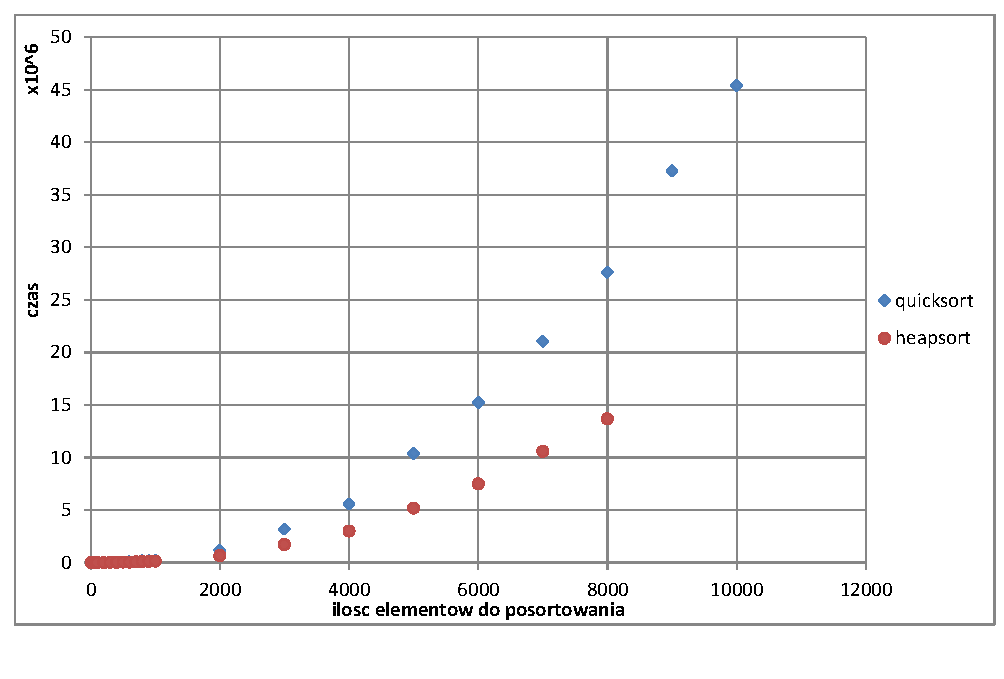
\includegraphics[scale=0.75]{wykres1.pdf}
\caption{Wykres złożoności obliczeniowej}
\label{fig:wykres1}
\end{figure}
\section{Uwaga}
Algorytm sortowania przez kopcowanie działa poprawnie dla tablicy alokowanej dynamicznie. Dla struktury typu lista, algorytm zawodzi :(. Powodem może być struktura, lecz quicksort działa jak powinien. Mimo to wykorzytano tę metode do sporządzenia wykresu, ponieważ operacje wykonywane przez algorytm nie są niepoprawne, a wykres jest tylko przybliżeniem.
\section{Komentarz}
Funkcja pomiaru czasu dla systemu Windows pobrana ze strony dr. J. Mierzwy. Program skompilowano w środowisku Code::Blocks. Do stworzonia wykresu posłużono się pakietem MS Excel, sprawozdanie napisano używając systemu \LaTeX.
\end{document}